\documentclass[12pt]{article}

% This first part of the file is called the PREAMBLE. It includes customizations and command definitions. The preamble is everything between \documentclass and \begin{document}.
\usepackage[top=0.75in, bottom=1.25in, left=1in, right=1in]{geometry} 
\usepackage{amsmath,amsthm,amssymb} %this is THE math package
\usepackage{mathtools}
\usepackage{tikz}
\usepackage{graphicx}
\usepackage{fancybox}
\usepackage{hyperref}
\usepackage{varwidth}
\usepackage{mdframed}
\usepackage{mathrsfs}
\usepackage[most]{tcolorbox}
\usepackage{xcolor}
%------------------------
%Fonts I use, uncomment if you like to use them.
%The first is the general font, and the second a math font
\usepackage{mathpazo}
\usepackage{eulervm}
%------------------------
%This is so that we have standard fonts for the double-stroked symbols
%for reals, naturals etc. regardless of what font you use.
%Don't comment
\AtBeginDocument{
  \DeclareSymbolFont{AMSb}{U}{msb}{m}{n}
  \DeclareSymbolFontAlphabet{\mathbb}{AMSb}}
%------------------------

\usepackage[english]{babel}
\usepackage{mathtools}
\usepackage{tikz-cd}


\newtheorem{thm}{Theorem}[section]
\newtheorem{lem}[thm]{Lemma}
\newtheorem{prop}[thm]{Proposition}
\newtheorem{cor}[thm]{Corollary}
\newtheorem{conj}[thm]{Conjecture}
\newtheorem{mydef}[thm]{Definition}

\theoremstyle{definition}
\newtheorem{definition}{Definition}[section]

\theoremstyle{remark}
\newtheorem*{remark}{Remark}

%----------------------------------------------
%User-defined environments
%Commented because we're not using them in this document
%The only uncommented ones are the Problem and Solution environment

% \newenvironment{theorem}[2][Theorem]{\begin{trivlist}
% \item[\hskip \labelsep {\bfseries #1}\hskip \labelsep {\bfseries #2.}]}{\end{trivlist}}
% \newenvironment{lemma}[2][Lemma]{\begin{trivlist}
% \item[\hskip \labelsep {\bfseries #1}\hskip \labelsep {\bfseries #2.}]}{\end{trivlist}}
% \newenvironment{exercise}[2][Exercise]{\begin{trivlist}
% \item[\hskip \labelsep {\bfseries #1}\hskip \labelsep {\bfseries #2.}]}{\end{trivlist}}
% \newenvironment{question}[2][Question]{\begin{trivlist}
% \item[\hskip \labelsep {\bfseries #1}\hskip \labelsep {\bfseries #2.}]}{\end{trivlist}}
% \newenvironment{corollary}[2][Corollary]{\begin{trivlist}
% \item[\hskip \labelsep {\bfseries #1}\hskip \labelsep {\bfseries #2.}]}{\end{trivlist}}
\newenvironment{problem}[2][Problem\!]{\begin{trivlist}
\item[\hskip \labelsep {\bfseries #1}\hskip \labelsep {\bfseries #2}]}{\end{trivlist}}
%\newenvironment{sub-problem}[2][]{\begin{trivlist}
%\item[\hskip \labelsep {\bfseries #1}\hskip \labelsep {\bfseries #2}]}{\end{trivlist}}
\newenvironment{solution}{\begin{proof}[\textbf{\textit{Solution}}] }{\end{proof}}
%----------------------------------------------

%----------------------------
%User-defined notations
\newcommand{\zz}{\mathbb Z}   %blackboard bold Z
\newcommand{\qq}{\mathbb Q}   %blackboard bold Q
\newcommand{\ff}{\mathbb F}   %blackboard bold F
\newcommand{\rr}{\mathbb R}   %blackboard bold R
\newcommand{\nn}{\mathbb N}   %blackboard bold N
\newcommand{\cc}{\mathbb C}   %blackboard bold C
\newcommand{\af}{\mathbb A}   %blackboard bold A
\newcommand{\pp}{\mathbb P}   %blackboard bold P
\newcommand{\id}{\operatorname{id}} %for identity map
\newcommand{\im}{\operatorname{im}} %for image of a function
\newcommand{\dom}{\operatorname{dom}} %for domain of a function
\newcommand{\cat}[1]{\mathscr{#1}}   %calligraphic category
\newcommand{\abs}[1]{\left\lvert#1\right\rvert} %for absolute value
\newcommand{\norm}[1]{\left\lVert#1\right\rVert} %for norm
\newcommand{\modar}[1]{\text{ mod }{#1}} %for modular arithmetic
\newcommand{\set}[1]{\left\{#1\right\}} %for set
\newcommand{\setp}[2]{\left\{#1\ \middle|\ #2\right\}} %for set with a property
\newcommand{\card}[1]{\#\,{#1}} %for cardinality of a set
\newcommand\m[1]{\begin{pmatrix}#1\end{pmatrix}} 

%Re-defined notations
\renewcommand{\epsilon}{\varepsilon}
\renewcommand{\phi}{\varphi}
\renewcommand{\emptyset}{\varnothing}
\renewcommand{\geq}{\geqslant}
\renewcommand{\leq}{\leqslant}
\renewcommand{\Re}{\operatorname{Re}}
\renewcommand{\Im}{\operatorname{Im}}
%----------------------------

\newcommand{\lrp}[1]{\left(#1\right)}
\newcommand{\lrb}[1]{\left[#1\right]}
\newcommand{\lrc}[1]{\left\{#1\right\}}

\newcommand{\tcr}[1]{\textcolor{red}{#1}}

\allowdisplaybreaks



\begin{document}


\title{P-adic Numbers}

\author{Kevin Guillen \\ 
Department of Mathematics \\
University of California at Santa Cruz \\
Santa Cruz, CA 95064 USA}

\maketitle

\begin{abstract}
This paper will begin by introducing some of the prerequisite knowledge and definitions needed to define $p-$adic numbers and their applications. This will be done by building them alongside the reals and providing the needed history. The main focus though is to give the motivation for their discovery, the intuition behind them, and proving Ostrowksi's theorem to enforce their importance. Exploring the definition of completion and the ring of $p$-adic integers. Finally exploring some unnatural properties of them. 
\end{abstract}

\section{Introduction}
The real numbers are a number system we should all be familiar with, since it is what appears most natural in our day to day lives. For one to construct the reals from the rationals though, it turns out to be difficult due to one needing more machinery than when going from the natural numbers $\nn$, to the integers $\zz$ and finally to the rationals $\qq$. In these two "jumps" one simply needed to introduce one more algebraic operation to get the next. For example one got the integers from the natural numbers through the introduction of subtraction, and the rationals from the integers through the introduction of division. The new machinery one needed to jump from the discrete $\qq$ to the continuous $\rr$ was the introduction of a limit $\lrb{4}$ . The standard definition of a limit in the real numbers depends on the standard notion of distance, the Euclidean absolute value, which is a \textit{metric} or a \textit{distance function}$\lrb{5}$. That's the key though, the Euclidean absolute value is \textit{a} metric, so while this paper is not on measure theory, this will be important for what comes next. We know that $\qq$ was a field and through the Euclidean absolute value we were able to obtain the reals, which now leads us to define the general notion of absolute value for an arbitrary field $\ff$.
\newpage
\begin{definition}[Absolute Value]
  An \textbf{absolute value} on a field $\ff$ is a function $\abs{\cdot}$ from $\ff$ to $\rr_{\geq 0}$ that satisfies the following properties for all $a,b \in \ff$:
  \begin{itemize}
    \item[(1)]Positive-definiteness: $\abs{a} = 0 \Longleftrightarrow a = 0$  
    \item[(2)]Multiplicativity: $\abs{ab} = \abs{a} \abs{b}$ 
    \item[(3)]Triangle Inequality: $\abs{a + b} \leq \abs{a} + \abs{y}$    
  \end{itemize}
  and if an absolute value satisfies,
  \begin{itemize}
    \item[(4)] Strong Triangle Inequality: $\abs{a + b} \leq \max\lrc{\abs{a}, \abs{b}}$
  \end{itemize}
  it is called \textit{non-Archimedean}.
\end{definition}
We also define a metric as follows,
\begin{definition}[Metric]
  A \textbf{metric} on $\ff$ is defined by a distance function $d: \ff \times \ff \to \rr_{\leq 0}$. We see then that an absolute value induces a metric by,
  \[d(a,b) = \abs{a - b}\]
  for all $a,b \in \ff$
  A set where a metric is defined is called a \textit{metric space}, and a set with a metric is induced by a non-Archimedean absolute value is called a \textit{ultrametric space}
\end{definition}

We see then that $(\rr, d)$ where $d$ is the usual Euclidean absolute value, we have a metric space that we all naturally know. 

What was the point of all this, why did we review these definitions and constructions? Well, there is a different number system one can obtain from the rationals that is just as, if not more, fascinating than the reals, and that is the \textit{p-adic} number system. 

\begin{definition} [p-adic integer]
  Let $p \in \zz$ be a prime number. Then a \textbf{$p$-integer} $x$ is the base $p$ expansion of some integer $a\in \zz$, that is,
  \begin{align*}
    a &= a_1p^{0} + a_2p^{1} + \dots + a_np^{n}  && a_1,a_2, \dots a_n \in \zz/p\zz\\
    x &= a_1a_2\dots a_n
  \end{align*}
\end{definition}
where we will define p-adic integers to be "closer" to one another based on how many powers of $p$ we can fit into their difference. This number system, even though unnatural, will prove to be a useful toolset and yield a number of fascinating and unintuitive results. We will touch on many familiar topics relating to the reals, and how those topics look like in this number system. We stop here since it will be good to see why how anyone would think of a number system and see the motivation behind its discovery.  

\section{Hensel's Analogy}
This definition/construction of $p-$adic numbers may seem a bit aimless and random, but once we see what was going through the mind of Hensel, we will see that this number system is indeed well motivated and natural. 

Kurt Hensel (29 December 1861 - 1 June 1941) was a German mathematician born in Konigsberg, who studied under Leopold Kronecker and Karl Weierstrass. At the time Hensel was interested in the analogy between,
\begin{align*}
  \zz \text{ with its fraction field } \qq \longleftrightarrow \cc[X] \text{ with its fraction field }\cc(X).
\end{align*}

Hensel learned of this analogy from his doctoral advisor Kronecker, who believed there could be a single theory covering both of them. Kronecker never was able to create this theory, but Hensel was very interested in this analogy between the two $\lrb{1}$. 

We can see how this interest through the following explanations. Taking a function $f(X)$ from $\cc(X)$ we know it is a rational function or in other words the quotient of two functions,
\begin{align*}
  f(X) = \frac{P(X)}{Q(X)}, \ P(X),Q(X) \in \cc[X].
\end{align*}
Taking a rational number $x$ from $\qq$ we know that it is rational, as the name suggests, more specifically a quotient of two integers,
\begin{align*}
  x = \frac{p}{q}, \ p,q \in \zz.
\end{align*}

The next parallel is that we know both the rings $\zz$ and $\cc[X]$ are unique factorization domains, meaning every non-zero non-unit element in them can be written uniquely as a product of prime elements in the ring (up order and units). More explicitly for $x \in \zz$ non-zero and not $\pm 1$ we can express it uniquely for $n \in \nn$ as,
\begin{align*}
  x = p_1^{e_1} p_2^{e_2}\dots p_n^{e_n}, \ p_1\dots p_n \text{  are prime integers}, \ e_1\dots e_n \in \nn
\end{align*}
And for $P(X) \in \cc[X]$ where $P(X)$ is non-zero and not a unit, we can express it uniquely, for some $n \in \nn$, as,
\begin{align*}
  P(X) = a(X - \alpha_1)(X-\alpha_2)\dots (X - \alpha_n), \ a,\alpha_1\dots\alpha_n \in \cc.
\end{align*}
From here one might be able to see what the point of Hensel's analogy was. It's that primes,$p$, in $\zz$ are analogous to linear polynomials, $(X-\alpha)$, in $\cc[X]$

Extending this into solutions for equations. If we take a polynomial with integer coefficients, we call its roots \textit{algebraic numbers}. Now something similar is said when we take a polynomial with coefficients in $\cc[X]$, its roots will be called \textit{algebraic functions}.

\textbf{Example}: Consider the polynomial $Y^{2}-2$, we know $\sqrt{2}$ is a root of it, and therefore $\sqrt{2}$ is an algebraic number. 

Now for the polynomial with coefficients in $\cc[X]$, $Y^{2} - (X^{3}-3X - 1)$ the function $\sqrt{X^{3}-3X -1}$ is a root of it, and therefore and algebraic function. 

Going back to Hensel's analogy now, Hensel was working on a specific problem about algebraic numbers, so he considered the analogous problem in terms of algebraic functions. This problem that Hensel was working on turned out to be relatively easy to solve under algebraic functions by expanding functions into its power series $\lrb{1}$. Explicitly this means, given $P(X) \in \cc[X]$ and $\alpha \in \cc$ we have the following,
\begin{align*}
  P(X) &= a_0 + a_1(X -\alpha)^{1} + a_2(X-\alpha)^{2} + \dots + a_n(X-\alpha)^{n} \\
  &= \sum_{i = o}^{n}a_i(X-\alpha)^{i}.
\end{align*}
Which gives us information of how $P(X)$ behaves around $\alpha$. Now if only we had this sort of expansion for integers. In a way we do though! Consider the number $245$, we can expand it out as follows,
\begin{align*}
  245 = \tcr{5}\cdot 10^{0} + \tcr{4}\cdot 10^{1} + \tcr{2} \cdot 10^{2}
\end{align*}
which is nothing new, we do it all the time we just stop thinking about it. The issue for Hensel though was that $10$ is not a prime in $\zz$ while $(X-\alpha)$ is a prime in $\cc[X]$. Knowing the definition of $p-$adic numbers we know what comes next. Hensel considered taking a base 10 integer and expressing it a number in base $p$. So we see our $245$ becomes,
\begin{align*}
  245 &= \tcr{1} \cdot 2^{0} + \tcr{1}\cdot 2^{1} + \tcr{1} \cdot 2^{2} + \tcr{1}\cdot 2^{3} + \tcr{0}\cdot 2^{4} + \tcr{1} \cdot 2^{5} + \tcr{0} \cdot 2^{6} + \tcr{1}\cdot 2^{7} \\
  &= \tcr{11110101}_2
\end{align*}
which we see is analogous to the power series for functions since $2$ is a prime element in $\zz$

\section{Properties of $p$-adic numbers}
Now that we see how Hensel arrived at $p$-adic numbers let us expand on some of the definitions given during the introduction and dive deeper into the world of $p-$adic numbers. We know from previously that we can simply take a base 10 integer and express it in base $p$, where $p$ is a prime number, and have its $p$-adic equivalent, but the $p$-adic numbers are supposed to be an extension of the rational numbers so let us consider a rational number $x$. We know that it is of the form $\dfrac{a}{b}$. To follow from the work of the previous section let $a = 245$ with $b = 4$ and lets work in the $2$-adic system. We know from perviously that $245$ is $\tcr{11110101}_2$ and we see that
\begin{align*}
  \dfrac{245}{4} &= \tcr{1} \cdot 2^{-2} + \tcr{0} \cdot 2^{-1} + \tcr{1} \cdot 2^{0} + \tcr{0} \cdot 2^{1} + \tcr{1}\cdot 2^{2} + \tcr{1} \cdot 2^{3} + \tcr{1} \cdot 2^{4} + \tcr{1} \cdot 2^{5} \\
  &= \tcr{111101.01}_2 
\end{align*} 
where the decimal behaves as normally in base 10. Technically there wasn't much if any calculations needed here since just like in base 10 when we are dividing by a power of $p$ we simply "move" the decimal point to the left based on what power of $p$ we are dividing by. In this case $4 = 2^{2}$. So in a sense this was trivial, but let us ease into some not as nice fractions. let us consider $\dfrac{1}{2}$ in the $5-$adic system. We get,
\begin{align*}
  \dfrac{1}{2} = 5 \cdot \dfrac{-1}{2} + \tcr{3}
\end{align*}
this tells us that 3 will be the last digit and we know it to be unique since $5$ is prime. Continuing this division with remainder we get,
\begin{align*}
  \dfrac{-1}{2} &= 5 \cdot \dfrac{-1}{2} + \tcr{2} \\
  \dfrac{-1}{2} &= 5 \cdot \dfrac{-1}{2} + \tcr{2} \\
  &\ \ \vdots
\end{align*}
and we see this process just repeats meaning $\dfrac{1}{2}$ in the $5-$adic system will simply be $\tcr{\dots223_5} = \tcr{\bar{2}3}_5$. This is the general idea of how to obtain the $p-$adic expansion of a rational number (note that the for an integer the $p-adic$ expansion is simply its expression in base $p$). There is a lot being tucked under the rug here, but in order to have time to talk about more advanced topics we will be omitting some little details. We see then that any rational number can expressed in the form,
\[x = \dfrac{a}{b} = \sum_{n\geq n_0}a_np^{n}\]
where $n_0 \geq 0 $ if and only if $p\nmid b$ and $n_0 > 0$ if and only if $p\nmid b$ AND $p \nmid a$ where we assume $\dfrac{a}{b}$ is in its lowest terms. 

Now let us return a bit to Hensel's Analogy, we see that for every rational number when converted to its $p-$adic expansion we will have finitely many negative powers of $p$. This is called a "finite-tailed Laurent series in $p$".$\lrb{1}$ Which is referencing the expansion is finite to the left (or finite to the right once we write it out in the specified base). Now we know that $\cc\lrp{\lrp{X - \alpha}}$ is a field, will the set of all finite tailed Laurent series in powers of $p$ be a field? The answer is yes! This field is actually refered to as $\qq_p$ which is said as the field of $p-$adic numbers.  Now that we got some basic concepts down we can actually dive into one of the problems that $p-$adic numbers are closely related to. 

\subsection{Solving Congruences Modulo $p^{n}$}
  Problems of these kind are common in a field like Number Theory, so to begin this let us consider an equation that has solutions in $\qq$,
  \[X^{2} = 16.\]
  Which has solutions $x = \pm 4$. Now we want to consider it modulo $p^{n}$ and $\forall n \in \nn$, in order to solve congruences like,
  \[X^{2} \equiv 16\text{ mod } p^{n}\]
  and for the integers we know that $X = \pm 4$ gives solutions of the congruence for every $n$. Want we want to do is consider it from a $p-$adic point of view. Let us consider specifically the $3-$adic system. Recall this means we will be writing with class representatives between 0 and $3^{n} -1$ for solutions modulo $3^{n}$. So first let us look at $X = 4$ we have,
  \begin{align*}
    X &\equiv 4 \equiv \tcr{1} \text{ mod }3^{1} \\
    X &\equiv 4 = \tcr{1} + \tcr{1}\cdot 3^{1} \text{ mod }3^{2} = 9 \\
    X &\equiv 4 = \tcr{1} + \tcr{1}\cdot 3^{1} \text{ mod }3^{3} = 27 \\
    & \ \  \vdots 
  \end{align*} which we see will continue on for the rest of the powers of $3$, giving the $3-$adic expansion of the solution as,
  \[4 = \tcr{1}\cdot 3^{0} + \tcr{1}\cdot 3^{1} = \tcr{11}_3\]
  let us consider the more interesting solution though, $X = -4$ we see that,
  \begin{align*}
    X&\equiv -4 \equiv 2  = \tcr{2}_3 \text{ mod } 3 \\ 
    X &\equiv -4 \equiv 5 = \tcr{2} + \tcr{1}\cdot 3^{1} = \tcr{12}_3 \text{ mod } 9 \\ 
    X & \equiv -4 \equiv 23 = \tcr{2} + \tcr{1} \cdot 3^{1} + \tcr{2}\cdot 3^{2} = \tcr{212}_3 \text{ mod } 27 \\
    X &\equiv -4 \equiv 77 = \tcr{2} + \tcr{1}\cdot 3^{1} + \tcr{2}\cdot 3^{2} + \tcr{2}\cdot 3^{3} = \tcr{2212}_3 \text{ mod } 81 \\
    & \ \ \vdots 
  \end{align*}
  continuing this as before gives the $3-$adic expansion of the solution which we see to be infinite!
  \[X = -4 = \tcr{2}\cdot 3^{0} + \tcr{1}\cdot 3^{1} + \tcr{2}\cdot 3^{2} + \tcr{2}\cdot 3^{3} + \dots  = \tcr{\dots2212}_3 = \tcr{\overline{2}12}_3 \]
  We see that the solutions for the congruencies are "coherent" meaning if we take the solution for $3^{4}$ which was $X = 77$ and reduce it modulo $3^{3}$ we get $X = 23$, which is the corresponding solution for $3^{3}$, which leads to a definition.

  \begin{mydef}(\textbf{Coherent})
    Let $p$ be a prime integer. A sequence of integers $\alpha_n$ such that $0 \leq \alpha_n \leq p^{n} -1 $ is \textbf{coherent} if for every $n \geq 1$ it satisfies,
    \[\alpha_{n+1} \equiv \alpha_n \text{ mod }p^{n}\]
    in the case where $p$ must be specified, the sequence will be called \textbf{$p$-adically coherent}. $\lrb{1}$
  \end{mydef}

  When we have a \textbf{coherent} sequence of integers we can visualize the solutions as a branch, let us consider specifically the solutions we worked out above $X = \pm 4$. 
  \[
  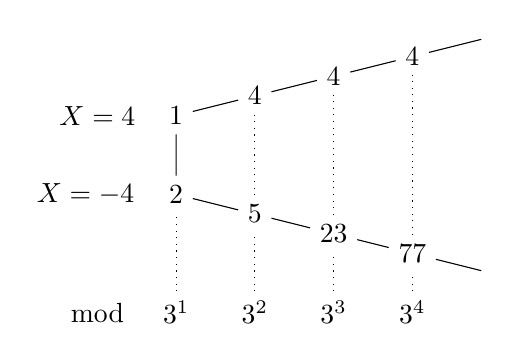
\begin{tikzpicture}
    \node (1) at (0,1) {$ 1$};
    \node (2) at (0,0) {$2$};
    
    \node (4) at (1,1.25) {$4$};
    \node (7) at (2,1.5) {$4$};
    \node (8) at (3, 1.75) {$4$};
    \node (9) at (4, 2) {};

    \node (5) at (1, -0.25) {$5$};
    \node (23) at (2,-.5) {$23$};
    \node (77) at (3, -.75) {$77$};
    \node  (88) at (4, -1){};

    \node (sol1) at (-1, 1) {$X = 4$};
    \node (sol2) at (-1.15, 0) {$X = -4$};

    \draw (4) -- (1) -- (2) -- (5) -- (23) -- (77) -- (88);
    \draw (4) -- (7) -- (8) -- (9);

    \node (z) at (-1, -1.5) {mod};
    \node (a) at (0, -1.5) {$3^{1}$};
    \node (b) at (1, -1.5) {$3^{2}$};
    \node (c) at (2, -1.5) {$3^{3}$};
    \node (d) at (3, -1.5) {$3^{4}$};

    \draw[dotted] (a) -- (2); \draw[dotted] (b) -- (5) -- (4); \draw[dotted] (c) -- (23) -- (7) ; \draw[dotted] (d) -- (77) -- (8);
  \end{tikzpicture}
  \]
  Anyone familiar with congruencies would know this was already obvious for these solutions since they are actually solutions in $\zz$, what is new is the connection between expressing the roots as coherent sequences containing their $p-$adic expansions. 

  To make it more interesting let us consider an equation that doesn't have solutions in $\qq$, a notable one to consider is,
  \[X^{2} = 2.\]
  Let us look at this under the $7-$adic lens,
  \begin{align*}
    X^{2} \equiv 2 \text{ mod } 7
  \end{align*}
  we obtain two solutions:
  \begin{align*}
    X \equiv 3 \text{ mod } 7 && X \equiv 4 \equiv -3 \text{ mod } 7. 
  \end{align*}
  Now let us continue like before and find solutions for $n =2$ or in other words 
  \[X^{2} \equiv 2 \text{ mod }49\]
  recall though to be \textbf{coherent}, these solutions reduced modulo 7 must also be solutions for $n = 1$. This gives us the requirements,
  \begin{align*}
    X = 3+ 7k && X = 4 + 7k
  \end{align*}
  so let us begin solving for the first solution, plugging it in gives us,
  \begin{align*}
    (3 + 7k)^{2} &\equiv 2 \text{ mod }49 \\
    9 + 42k &\equiv 2 \text{ mod }49  \\
    7(1 + 6k)= 7 + 42k &\equiv 0 \text{ mod }49 \\
    1 + 6k & \equiv 0 \text{ mod }7 \\
    k &\equiv 1 \text{ mod }7.
  \end{align*}
  By definition this gives us then that, $k = 7m + 1$ where $m \in \zz$. Plugging this back into $X$ gives us that $X = 10 + 49m$, meaning this solution for $n = 2$ is,
  \[X \equiv 10 \text{ mod } 49. \]
  Similarly we obtain the second solution in the same fashion which works out to be, \[X \equiv 39 \equiv -10 \text{ mod }49.\]

  From here one repeat these steps for $n = 3,4,5\dots$ to then create the branches that we saw before. It should be noted though that this is not a way to predict numbers will appear in the branch, but what this repetition does tell us though is that we can find two coherent sequences of solutions. $\lrb{1}$ 
  \[ 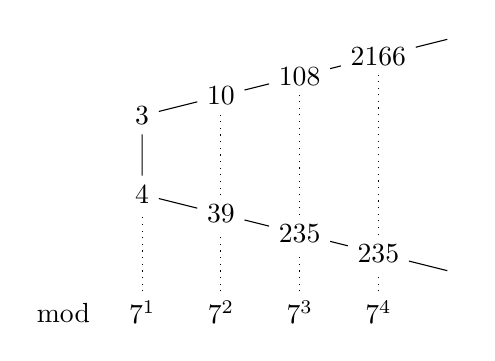
\begin{tikzpicture}
    \node (1) at (0,1) {$ 3$};
    \node (2) at (0,0) {$4$};
    
    \node (4) at (1,1.25) {$10$};
    \node (7) at (2,1.5) {$108$};
    \node (8) at (3, 1.75) {$2166$};
    \node (9) at (4, 2) {};

    \node (5) at (1, -0.25) {$39$};
    \node (23) at (2,-.5) {$235$};
    \node (77) at (3, -.75) {$235$};
    \node  (88) at (4, -1){};

    \draw (4) -- (1) -- (2) -- (5) -- (23) -- (77) -- (88);
    \draw (4) -- (7) -- (8) -- (9);

    \node (z) at (-1, -1.5) {mod};
    \node (a) at (0, -1.5) {$7^{1}$};
    \node (b) at (1, -1.5) {$7^{2}$};
    \node (c) at (2, -1.5) {$7^{3}$};
    \node (d) at (3, -1.5) {$7^{4}$};

    \draw[dotted] (a) -- (2); \draw[dotted] (b) -- (5) -- (4); \draw[dotted] (c) -- (23) -- (7) ; \draw[dotted] (d) -- (77) -- (8);
  \end{tikzpicture}\]
  Which gives us the sequence of integers,
  \begin{align*}
    \alpha_1 &= (3, 10, 108, 2166, \dots) \\
    \alpha_2 &= (4, 39, 235, 235, \dots)
  \end{align*}
  as our solutions, and now repeating what we did previous we can obtain the $7-$adic expansion of the solution,
  \begin{align*}
    3 &= 3 = \tcr{3}_7 \\
    10 &= \tcr{3} + \tcr{1}\cdot 7^{1} = \tcr{13}_7 \\ 
    108 &= \tcr{3} + \tcr{1}\cdot 7^{1} + \tcr{2}\cdot 7^{2} = \tcr{213}_7 \\
    2166 &= \tcr{3} + \tcr{1}\cdot 7^{1} + \tcr{2}\cdot 7^{2} + \tcr{6}\cdot 7^{3}= \tcr{6213}_7
  \end{align*}
  meaning the $7-$adic solutions are simply,
  \begin{align*}
    \alpha_1 = \tcr{\dots 6213}_7 \\
    \alpha_2 = \tcr{\dots 0454}_7.
  \end{align*}
  So we could continue this methodology infinitely to keep obtaining the rest of the solution, since we can't predict what the rest of the solution will look like with what we have currently. Think of this similar to how we can work out the decimal expansion of the square root of $2$ in $\rr$ and get as close as we'd like, but we can't predict what the expansion will look like. $\lrb{3}$ Finally these two $7-$adic numbers are the roots of the equation $X^{2} = 2$ in the field of $7-$adic numbers, $\qq_7$. These sequences of congruences modulo higher and higher powers of $p$ and solving the corresponding equation in $\qq_p$ are of the important reasons for using $p-$adic methods in Number Theory. $\lrb{1}$ This leads beautifully into the next important topic pertaining to $p-$adic numbers and that is completion, which is why we chose the example of $X^{2} = 2$.

\section{Completing $\qq$}
  Let us bring in some of the definitions defined in the introduction. One might have picked up why they were defined, since they in a way served as a spoiler for what is to come especially after showing some properties of the $p-$adics. First we will bring in a few other definitions. 
  \begin{mydef}(\textbf{Cauchy Sequence} $\lrb{4}$) A sequence $(x_n)$ is a \textbf{Cauchy} if $\forall \epsilon > 0$ there exists some $N \in \nn$ such that for all $n,m > N$ it satisfies,
    \[\abs{x_n - x_m} < \epsilon.\]
  \end{mydef} 
  When a sequence is Cauchy, all it is really saying about the sequence is that the terms in the sequence become arbitrarily close to one another and in a sense "settle" on something. Which is why the convergence of a sequence implies it is Cauchy. $\lrb{4}$

  \begin{mydef} (\textbf{Complete})
    A metric space is called \textbf{complete} if every Cauchy sequence composed of elements in the metric space converges within the metric space. Such a metric space is also referred to as a \textbf{Cauchy Space}. $\lrb{5}$
  \end{mydef}

  \begin{remark}
    The field $\qq$ is NOT complete. Recall we simply have to show an example of one Cauchy sequence composed of rational numbers that converges to something not in $\qq$. One example would be,
    \[x_n = \lrp{1 + \dfrac{1}{n}}^{n}\]
    which one can prove is convergent to $e$, therefore Cauchy, but $e \notin \qq$. This leads one to construct the reals, $\rr$, in order to complete $\qq$ under the standard Euclidean absolute value. 
  \end{remark}

  Now we may wonder what other metrics (distance functions) we can impose on $\qq$ and what number systems may come from there. In fact the field of $p-$adic numbers can be analytically constructed through this. This leads to the formal construction of $\qq_p$, by defining the $p-$adic absolute value, but first we must define $p-$adic valuation.

  \begin{mydef} (\textbf{P-adic valuation} $\lrb{1}$)
    $P-$adic valuation is defined as the map,
    \begin{align*}
      v_p: \qq \to \zz \cup \set{\infty} \\
    \end{align*}
    where if $x \in \zz$, then $v_p(x)$ is the unique positive integer satisfying,
    \[x = p^{v_p(x)}x'\]
    where $p \nmid x'$.

    If $x \in \qq- \zz$ then $x$ is of the form $x = \dfrac{a}{b}$ where $a,b \in \zz$, so $v_p(x)$ is defined to be,
    \[v_p(x) = v_p(a) - v_p(b).\]

    Lastly we define $v_p(0) = \infty$ (the reason will be more obvious soon). 
  \end{mydef}

  \textbf{Example.} First lets cover an integer example, so let $x = 90$ and $p = 3$. The $3-$adic evaluation of $90$ will be $2$ since,
  \[90 = 3^{2}\cdot 10.\]
  Now consider the case $x = \dfrac{13}{24}$ and $p = 2$. So we have $v_2(13) = 0$ since we can't factor out any non-zero powers of $2$, and $v_2(24) = 3$ since we can factor out $8$. This means,
  \[v_2\lrp{\dfrac{13}{24}} = v_2(13) - v_2(24) = 0 -3 = -3.\]
  
  With this we can now define the $p-$adic absolute value.

  \begin{mydef}(\textbf{P-adic absolute value} $\lrb{1}$)
    The $p-$adic absolute value is a function,
    \[\abs{\cdot}_p: \qq \to \rr_{\geq 0}\]
    defined as,
    \begin{align*}
      \abs{x}_p = \begin{cases}
        p^{-v_p(x)} & x \neq 0 \\
        0 & x = 0
      \end{cases}
    \end{align*}
    where $p$ is a prime integer. 
  \end{mydef}
    \begin{prop}
      The $p-$adic absolute value is a non-Archimedean absolute value on $\qq$.
    \end{prop}
    \begin{proof} Let $x,y \in \qq$,
      \begin{itemize}
        \item[(1)] If $\abs{x}_p = 0$ then by definition 4.4, $x = 0$
        \item[(2)] If $x = 0$ or $y = 0$ then it is obvious that $\abs{xy}_p = \abs{x}_p\abs{y}_p$. Now in the case that $x \neq 0$ and $y \neq 0$ we have
        \begin{align}
          \abs{xy}_p = p^{-v_p(xy)} && \abs{x}_p\abs{y}_p = p^{-v_p(x) -v_p(y)}
        \end{align} 
        so we have to show that $v_p(xy) = v_p(x) + v_p(y)$.
        \begin{lem}
          \[v_p(xy) = v_p(x) + v_p(y)\]
        \end{lem}
        \begin{proof}
          Recall the definition of the $p-$adic valuation \textbf{Definition 4.3} and apply to it $x,y$ individually we get,
          \begin{align*}
            x = p^{v_p(x)}x' && y = p^{v_p(y)}y'
          \end{align*}
          therefore,
          \begin{align*}
            xy = p^{v_p(x)}x'p^{v_p(y)}y' = p^{v_p(x) + v_p(y)}x'y'
          \end{align*}
          by \textbf{Definition 4.3} $p \nmid x'$ and $p \nmid y'$, thus $p \nmid x'y'$. So we have that \[v_p(xy) = v_p(x) + v_p(y)\] since it satisfies,
          \[xy = p^{v_p(xy)}(xy)'\]
        \end{proof}
        Now applying \textbf{Lemma 4.6} $-v_p(xy) = -v_p(x) -v_p(y)$. All together then we have,
        \begin{align*}
          \abs{xy}_p = p^{-v_p(xy)} = p^{-v_p(x) -v_p(y)} = \abs{x}_p\abs{y}_p
        \end{align*}
        satisfying the multiplicativity requirement. 
        \item[(3)] Now to verify the triangle inequality and strong triangle inequality, if $x + y = 0 $ then it is obvious that $\abs{x + y}_p = 0$ and therefore $\abs{x +y }_p \leq \abs{x}_p + \abs{y}_p \leq \max\lrc{\abs{x}_p, \abs{y}_p}$.
        
        So let us consider the case that $x+y \neq 0$ and without loss of generality that $\abs{x}_p > \abs{y}_p$, and therefore $\abs{x}_p \neq 0 \neq x$. It follows then that $v_p(x) \leq v_p(y)$ and by \textbf{Definition 4.4} we have,
        \begin{align*}
          \abs{x + y}_p = p^{-v_p(x + y)} && \abs{x}_p = p^{-v_p(x)}
        \end{align*}
        To complete this we need,
        \begin{lem}
          \[v_p(x+ y) \geq \max\lrc{v_p(x), v_p(y)}\]
        \end{lem}
        \begin{proof}
          See $\lrb{2}$
        \end{proof}
        So applying \textbf{Lemma 4.7} we have,
        \[v_p(x + y) \geq \max\lrc{v_p(x), v_p(y)} = v_p(x)\]
        therefore,
        \[p^{-v_p(x + y)} \leq p^{-v_p(x)}\]
        which means then that,
        \[\abs{x + y}_p \leq \abs{x}_p = \max\lrc{\abs{x}_p, \abs{y}_p}.\]
      \end{itemize}

      All together then we have that the $p-$adic absolute value is non-Archimedean on $\qq$. 
    \end{proof}

    Let us take a pause here and answer some questions. We were able to motivate the field of $p-$adic numbers with Hensel's Analogy, and see why one would want such a number system. Right now though, depending on the person, one might feel this $p-$adic absolute value seems forced, or randomly made up. Why care about different absolute values, why not just stick to the traditional absolute value? One may also wonder if there are other absolute values we can define on $\qq$. This leads to a very important theorem that puts the $p-$adic value on the same level as the standard absolute value, and to be considered just as natural. 
\newpage
    \begin{thm} (\textbf{Ostrowski's Theorem} $\lrb{1}$) Every non-trivial absolute value on $\qq$ is equivalent to one of the absolute values $\abs{\cdot}_p$ where $p$ is either a prime integer or $p = \infty $ (the absolute value of the real numbers)
    \end{thm}
    That is to say an absolute value on the rational must fall under one of these three,
    \begin{align*}
      \abs{\cdot}_0 &= \begin{cases}
        0 & x = 0 \\
        1 & x = \neq 0
      \end{cases} \\
      \abs{\cdot}_\infty &= \begin{cases}
        x & x\geq 0 \\
        -x & x < 0 
      \end{cases} \\
      \abs{\cdot}_p &= \begin{cases}
        p^{-v_p(x)} & x \neq 0 \\
        0 & x = 0
      \end{cases}
    \end{align*}
    \begin{proof}
      Let us consider two cases for a non-trivial absolute value, where it is Archimedean and where it is non-Archimedean.
      \begin{itemize}
        \item[(1)] $\abs{\cdot}$ is Archimedean. Let us consider the least positive integer $x_0$ such that $\abs{x_0} > 1$, we know such an integer has to exist because if not this absolute value would be non-Archimedean. This means then that we can find an $\alpha \in \rr$ that will satisfy the following,
        \[\abs{x_0} = x_0^{\alpha}.\] 
        Now we claim that this $\alpha$ will realize the equivalence between $\abs{\cdot}$ and $\abs{\cdot}_\infty$. So all that we have to prove now is that for every $y \in \qq $ we have $\abs{y} = \abs{y}_\infty ^{\alpha}$, but knowing the properties of absolute values we simply have to show it for all positive integers $n \in \zz_+$ that $\abs{n} = \abs{n}_\infty ^{\alpha}$ since the rationals will follow from that. We know the equality will hold for $ x = x_0$, but to prove it in general, we can take an arbitrary integer $x$ and write it in base $x_0$ so to have in the form,
        \[x = a_0 + a1x_0 + a_2x_0^{2} + \dots + a_kx_0^{k}.\]
        where we have $0 \leq a_i \leq x_0 - 1$ and $a_k \neq 0$. We see though that $k$ is determined by $x_0 \leq x < x_0^{k+1}$, which says that,
        \begin{align*}
          k = \left\lfloor \dfrac{\log{x}}{\log{x_0}}\right\rfloor 
        \end{align*} 
        Now let us take the absolute values and we get,
        \begin{align*}
          \abs{x} = \abs{a_0 + a_1x_0 + a_2x_0^{2} + \dots a_kx_0^{k}} && \text{applying triangle inequality } \\
          \leq \abs{a_0} + \abs{a_1}x_0^{\alpha} + \abs{a_2}x_0^{2\alpha} + \dots + \abs{a_k}x_0^{k\alpha}         
        \end{align*}
        Now recall that $x_0$ is the smallest integer such that $\abs{x_0} > 1 $, we know then that $\abs{a_i} \leq 1$ and we get,
        \begin{align*}
          \abs{x} &\leq 1 + x_0^{\alpha} + x_0^{2\alpha} + \dots + x_0^{k\alpha} \\
                  &= x_0^{k\alpha}\lrp{1 + x_0^{-\alpha} + x_0^{-2\alpha} + \dots + x_0^{-k\alpha}} \\
                  &= x_0^{k\alpha}\sum_{i = 0}^{k}x_0^{-i\alpha} \\
                  &\leq x_0^{k\alpha}\sum_{i = 0}^{\infty}x_0^{-i\alpha} \\
                  &= x_0^{k\alpha}\dfrac{x_0^{\alpha}}{x_0^{\alpha}-1}
        \end{align*}
        Now it's obvious that $\dfrac{x_0^{\alpha}}{x_0^{\alpha}-1}$ is positive, and so let $C = \dfrac{x_0^{\alpha}}{x_0^{\alpha}-1}$, so now we have,
        \[\abs{x} \leq Cx_0^{k\alpha} \leq Cx^{\alpha}.\]
        This applies to every $x$ since our choice was arbitrary, now let us apply it to an integer of the form $x^{N}$ and we see we get,
        \[\abs{x^{N}} \leq Cx^{N\alpha}\]
        Recall that $C$ did not depend on the choice of $x$, so we can consider taking the $N$th root to obtain,
        \[\abs{x} \leq \sqrt[N]{C} \cdot x^{\alpha}. \]
        Now as $N\to \infty$ we have that $\sqrt[N]{C} \to 1$, meaning $\abs{x} \leq \abs{x}^{\alpha}$ which is part of what we want! So now we just need to show the reverse inequality, so let's consider $x$ written in base $x_0$ again,
        \[x = a_0 + a_1x_0 + a_2x_0^{2} + \dots + a_kx_0^{k}.\]
        Using the fact that $x_0^{k+1} > x \geq x_0^{k}$ we get,
        \[x_0^{(k+1)\alpha} = \abs{x_0^{k+1}} = \abs{x + x_0^{k+1} - x} \leq \abs{x} + \abs{x_0^{k+1} -x} \]
        so that,
        \[\abs{x} \geq x_0^{(k+1)\alpha} - \abs{x_0^{k+1} -x} \geq x_0^{(k+1)\alpha} - (x_0^{k+1} - x)^{\alpha}.\]
        Recall though that $x \geq x_0^{k}$ so we get,
        \begin{align*}
          \abs{x} \geq x_0^{(k+1)\alpha} - (x_0^{k+1} -x_0^{k})^{\alpha} = x_0^{(k+1)\alpha}\lrp{1 - \lrp{1 - \dfrac{1}{x_0}}^{\alpha}}
        \end{align*}
        Now similar to before let $C_1 = 1 - \lrp{1 - \dfrac{1}{x_0}}^{\alpha}$ which we see is not dependent on our choice of $x$ and wil be positive. This gives us,
        \begin{align*}
          \abs{x} \geq C_1x_0^{(k+1)\alpha} > C_1x^{\alpha}
        \end{align*}
        Like before we apply the same reasoning to get the reverse inequality, and therefore have that $\abs{x} = \abs{x}_\infty ^{\alpha}$. Thereby proving any Archimedean absolute value one can construct that is not the trivial one will be equivalent to $\abs{\cdot}_\infty$ as desired.
        \item[(2)] Now suppose we have an absolute value, $\abs{\cdot}$ that is not Archimedean, then every integer $x$ must have the result that $\abs{x} \leq 1$. Now because $\abs{\cdot}$ is non-trivial we have that there must be a smallest integer, $x_0$ such that $\abs{x_0} < 1$. First consider the case that $x_0 = bk$ where $b,k < x_0$, then by how $x_0$ was defined we have that $\abs{b} = \abs{k} = 1$ and that $\abs{bk} = \abs{x_0} < 1$ which cannot be. Therefore we have that $x_0$ must actually be prime! So, let us use traditional notation and let $p = x_0$. Now we want to show that this absolute value is actually equivalent to the $p-$adic absolute value. 
        
        Now our goal is to show that for any integer $k\in\zz$ that is not divisible by $p$ then $\abs{k} = 1$. To do this, we know if we divide $k$ by $p$ then through division with remainder we have,
        \[k= ap + b\]
        where $0 < b < p$. Recall we defined $p$ through $x_0$ and so $p$ is minimal. Then by the minimality of $p$ we have that $\abs{b} = 1$, and that $\abs{qp} < 1$, because $\abs{a} \leq 1$ ($\abs{\cdot}$ was assumed to be non-Archimedean and $\abs{p} < 1$ through construction). Now because $\abs{\cdot}$ is non-Archimedean we have that $\abs{k} = 1$. Therefore given any $k\in \zz$, we write it as $k = p^{v }k'$ where $p\nmid k'$. Then we have that,
        \[\abs{k} = \abs{p}^{v}\abs{k'} = \abs{p}^{v} = c^{-v}\]
        where we have $c= \abs{p}^{-1} > 1$. Meaning $\abs{\cdot}$ is equivalent to the $p-$adic absolute value. Completing the proof of Ostrowski's Theorem.
      \end{itemize}
    \end{proof}

    Hopefully this shows that the $p-$dic absolute value can be considered as natural as the standard absolute value. Here is a good place to expand on the shift of notation by using $\abs{\cdot}_\infty$ as the "usual" absolute value. If we think of $\infty$ as an infinite "prime", we can consider all absolute values on $\qq$ coming from a finite or an infinite prime $\lrb{2}$. 

    There are many contexts in arithmetic that it is considered useful to work with "all primes". Meaning it is useful to use the information obtained from all the absolute values that arise from $\qq$. One can think of $\abs{\cdot}_\infty$ ($\rr$'s absolute value) as recording information relating to the sign, while other absolute values record information relating to a variety of primes $\lrb{3}$. 

    \begin{thm} Let $\mathbb{K}$ be a field with an absolute value $\abs{\cdot}$. Then there exists a complete field $\mathbb{K}$' with an absolute value $\abs{\cdot}'$ that extends $\mathbb{K}$. The completion $\mathbb{K}'$ is unique up to isomorphism. Moreover, on $\mathbb{K}$, $\abs{\cdot}'$ restricts to $\abs{}$, and $\mathbb{K}$ is dense in $\mathbb{K}'$.
    \end{thm}
    \begin{proof}
      See $\lrb{2}$.
    \end{proof}

    This finally leads us to the field of $p-$adic numbers.
    \begin{mydef} (\textbf{Field of $p$-adic numbers} $\qq_p$ $\lrb{1}$) The field of $p-$adic numbers, denoted $\qq_p$, is defined as the completion of $\qq$ under the $p-$adic metric. We know this completion to exist and be unique by \textbf{Theorem 4.9}.
    \end{mydef}

    Which is what we have been building towards! From here we can also define the ring of $p-$adic integers, denoted by $\zz_p$, but some things should be mentioned first. This construction was through an analytic lens, but the field of $p-$adic numbers can also be constructed by first algebraically constructing the ring of $p-$adic integers and then considering its fraction fraction field, which will end up being $\qq_p$. Similar to how we can construct $\qq$ from $\zz$. 
    
    It should also be clear that due to \textbf{Theorem 4.8} and \textbf{Theorem 4.9}, the field $\rr$ and $\qq_p$ are the only completions of $\qq$!

    \subsection{Completing $\zz$}
    The title of this subsection may seem a bit strange to someone exposed to a bit of real analysis. Since any Cauchy sequence constructed by integers converges to an integer. This is because Cauchy sequences of integers are, boring. To anyone unfamiliar as to why, recall a sequence is Cauchy when the terms in the sequence become arbitrarily close to one another, but integers are at least "1 away" from one another. This means the only way to construct a Cauchy sequence of integers is to let the sequence be a constant sequence, meaning each term in the sequence is the same, making them uninteresting. Recall though we have a new metric, the $p-$adic metric, meaning we have a new notion of distance. Under the $p-$adic metric, integers can become arbitrarily close to one another!

    \begin{mydef} (Ring of $p-$adic integers $\zz_p$. $\lrb{1}$) The ring of $p-$adic integers, denoted by $\zz_p$, is defined as,
      \[\zz_p = \lrc{x \in \qq_p \mid \abs{x}_p < 1}\]
    \end{mydef}

    Like before, $\zz_p$ is the completion of $\zz$, this is because under our new metric we can find Cauchy sequences of integers that converge outside of $\zz$. 

\section{Exploring $\qq_p$}
    Now that we've achieved our main goal of defining the field of $p-$adic numbers and the motivation behind them, let's explore them and see how they compare to what we are familiar with. 

    \begin{thm}
      Let $(x_n)$ be a sequence in $\qq_p$, $(x_n)$ is Cauchy if and only if $\forall \epsilon >0$, there exists $N \in \nn$ such that $\forall n \geq N$ we have,
      \[\abs{x_{n+1} - x_n} < \epsilon.\]
    \end{thm}
    \begin{proof}
      ($\Rightarrow$) Assuming $(x_n)$ is Cauchy. Let $\epsilon > 0$, then there exists $N\in \nn$ such that for all $n,m \geq N$ we have,
      \[\abs{x_n - x_m}_p < \epsilon.\] Let $n\geq N$, then it is obvious that $n+1 \geq N$ and we have,
      \[\abs{x_{n+1} - x_n}_p < \epsilon\] proving the forward direction. 

      ($\Leftarrow$) Now we assume that for every $\epsilon > 0$ there exists some $N\in \nn$ such that for all $n \geq N$ we have,
      \[\abs{x_{n+1} - x_n}_p < \epsilon.\]
      Now let $n,m \geq N$, in the case that $n=m$ we have,
      \[\abs{x_n - x_m}_p = \abs{0}_p = 0 < \epsilon\]
      so let us consider when $n\neq m$. Without loss of generality let $n > m$, we then have $n = m + a$ for some $a \in \zz$. Therefore we can write $\abs{x_n - x_m}_p$ as,
      \[\abs{(x_{m+a} - x_{a + m -1}) + (x_{m+a - 1} - x_{a + m -2}) + \dots + (x_{m+1} - x_{ m})}_p\]
      recall though that the $p-$adic absolute value is non-Archimedean so,
      \[\abs{x_n - x_m}_p \leq \max\lrc{\abs{x_{m+i} - x_{m-i -1}}_p : i = 1,\dots,k}.\]
      We have then for some $i_0$, $1 \leq i_0 \leq k$,
      \[\abs{x_{m + i_0} - x_{m + i_0 - 1}}_p = \max\lrc{\abs{x_{m+i} - a_{m+i -1}}_p : i = 1, \dots , k}\]
      Meaning we have $\abs{x_n - x_m}_p \leq \abs{x_{m+ i_0} - x_{m + i_0 -1}}_p$. Note though that $m \geq N$, then through our assumption we have,
      \[\abs{x_{m + i_0} - x_{m + i_0 - 1}}_p < \epsilon.\]
      Then through transitivity we have that
      \[\abs{x_n - x_m}_p < \epsilon\]
      making $(x_n)$ Cauchy as desired. 
    \end{proof}

    Let us consider something a bit more interesting though. Maybe you've seen a sum that goes like,
    \[\sum_{i=1}^{\infty} = \dfrac{-1}{12}\]
    which is actually only true if using a different definition of summation, specifically Ramanujan Summation. Since under standard definitions the sum of all natural numbers is actually divergent. Similarly to this,
    \[\sum_{n= 0}^{\infty}2^{n}\]
    or not? Of course it is divergent under the standard definition of summation and working with the integers, but what if I told you that under the $2-$adic system this sum actually converged to something, specifically -1! We will prove this, by proving something more general.
    \newpage
    \begin{lem}
      Under the $p-$adic number system, $\sum_{n= 0}^{\infty}p^{n}$ converges and its sum is $\dfrac{1}{1-p}$.$\lrb{3}$
    \end{lem}
    \begin{proof}
      Let $(x_n)$ be the sequence of partial sums for $\sum_{n=0}^{\infty}p^{n}.$ Then for all $n \in \nn_0$ we have,
      \[x_n = \sum_{i = 0}^{n -1}p^{i}.\] It can be seen that,
      \[(1-p)\sum_{i=0}^{n-1}p^{i} = 1^{n} -p^{n}.\]
      Therefore,
      \[x_n = \sum_{i = 0}^{n-1}p^{i} = \dfrac{1-p^{n}}{1-p}.\]
      Notice now that,
      \[\lim_{n\to \infty} \dfrac{1}{1-p} = \dfrac{1}{1-p}\]
      but since we are in the $p-$adic system it can be easily verified that $\lim_{n\to \infty}p^{n} = 0$. Now all together we have,
      \[\lim_{n\to \infty} x_n = \lim_{n\to \infty}\dfrac{1}{1-p} - \lim_{n\to\infty}\dfrac{1}{1-p}\cdot\lim_{n\to\infty}p^{n} = \dfrac{1}{1-p} \]
      as desired
    \end{proof}
    Meaning under the $p-adic$ number system we can take the infinite sum of powers of $p$ and it will not only converge, but converge to something negative! This is very different from what we are used to. This also reveals why under the $p$-adic metric the integers are not complete since we created a sequence of partial sums where each term is an integer and is converging to something outside of $\zz$ (at least for $p> 2$) $\lrb{2}$.

    Another thing to note is that this is analogous the formula of a geometric series in $\rr$. Recall though that only held true where $\abs{x} <1$. Through similar reasoning this can also be extended to hold for all $x\in \qq_p$ that satisfy $\abs{x}_p < 1$. $\lrb{3}$ 

\section{Conclusion}
    We were able to construct the field of $p-$adic numbers in a more natural way to show them similarly to the reals, while at the same time contrasting their differences. Hopefully through the exposure of Ostrowski's Theorem one can see the importance of these numbers and explore them further! Their uniqueness is also matched greatly by their utility. One important mathematical object needed in Andrew Wiles' proof of Fermat's Last Theorem was $p$-adic numbers. They are also being explored in elliptical curve cryptography by considering an elliptical curve over the field of $p-$adic numbers. There use has also been found by physicists who are exploring $p-$adic quantum mechanics. Unfortunately we weren't able to touch on some very interesting geometric or topological properties of $p-$adic numbers, but hopefully one is motivated enough to go explore those through the references provided. We also weren't able to go over some visualization of a "$p-$adic number line", but the presentation that accompanies this paper goes into that. Thank you for reading.

\newpage
\begin{thebibliography}{9}
    \bibitem{texbook}
    Fernando Gouvea (2003) \emph{p-adic Numbers: An Introduction}, Springer Science \& Business Media, 2003.
    
    \bibitem{texbook}
    Alain M. Robert (2000) \emph{A Course in p-adic Analysis}, Springer; 2000th edition

    \bibitem{texbook}
    Svetlana Katok (2007) \emph{P-adic Analysis Compared With Real (Student Mathematical Library)}, American Mathematical Society
    
    \bibitem{texbook}
    Terence Tao (2016) \emph{Analysis I: Third Edition}, Hindustan Book Agency, 1st ed. 2016 edition

    \bibitem{texbook}
    James Munkres (2000) \emph{Topology}, Pearson College Div; 2nd edition (January 7, 2000)

    \bibitem{}
    David A. Madore (2000) \emph{A First Introduction to $p$-adic numbers}, http://www.madore.org/~david/math/padics.pdf
  \end{thebibliography}
\end{document}
